%Vector Boson Fusion (VBF) and other production mechanisms of Higgs Boson normally differ as regards the jet kinematics. 
Higgs production through fusion of vector bosons (VBF) and through other mechanisms normally differ as regards the jet kinematics.
%In this analysis, jets are thus used for the event categorization, which will be introduced in Section~\ref{sec:categorization}.

\subsubsection{Jet Identification}

Jets are reconstructed through anti-$k_T$ clustering algorithm out of particle-flow candidates, with distance parameter $R = 0.4$, 
after rejecting the charged hadrons that are associated with a pileup primary  vertex.

To reduce instrumental background, the tight working point jet ID suggested by the JetMET Physics Object Group is applied~\cite{JetID2018}. 
In addition, jets from Pile-Up are rejected using the PileUp jet ID criteria suggested by the JetMET POG~\cite{JetPUID2017}. 
In this analysis, the jets from within $|\eta| < 4.7$ area are required to have a transverse momentum greater that 30 GeV. 
In addition, jets are cleaned from any of the tight leptons (passing the SIP and isolation cut computed after FSR correction) 
and FSR photons by a separation criterion: $\Delta R(\text{jet,lepton/photon}) > 0.4$.

\subsubsection{Jet Energy Corrections}

The capability of current calorimeter to measure the energy of jets correctly is not linear.
Hence the measured energy cannot be regarded as particle's true energy and we need to estimate corrections to Jet Energy.
In the analysis, standard jet energy corrections are implemented to the reconstructed jets,
which consist of L1 Pileup, L2 Relative Jet Correction,
L3 Absolute Jet Correction for both Monte Carlo samples and data,
and also residual calibration for data~\cite{JECMC2018}. Jet Energy resolution corrections are also applied to MC.
%\textbf{At the moment only preliminary version of JEC for MC is available. As recommended no JEC is applied to data.}


\subsubsection{B-tagging}

In order to distinguish whether a jet is b-jet or not \emph{DeepCSV} algorithm is used as our b-tagging algorithm. It combines the same information as the previous tagger \emph{CSVv2} i.e. SIP, jet kinematics and  secondary vertex but uses information of more tracks. Also, the b-tag output discriminator is computed with a Deep Neural Network. 
In the analysis, a jet is considered as a b-tagged if it meets requirement of \emph{medium} working point, i.e. if its \verb |pfDeepCSVJetTags:probb + pfDeepCSVJetTags:probbb| discriminator is greater than 0.4184~\cite{BTAG2018}.

Scale factors of data to simulation efficiencies for b-tagging are provided for this working point for the full dataset varied in jet $\pt$, $\eta$ and flavour.
They are applied to simulated jets by downgrading (upgrading) the b-tagging status of a fraction of the b-tagged (untagged) jets that have a scale factor smaller (larger) than one. % \textbf{They are not yet available but will be applied as soon as they arrive.}


\subsubsection{Validation on data}
Similarly to what was done with electrons and muons, some validation studies are performed to probe agreement of data with simulated samples for jets. 
Events containing $\Zee$ or $Z\rightarrow\cP\mu^{+}\cP\mu^{-}$ were selecting, following the same trigger and lepton selection criteria of the main analysis, but increasing the $p_T$ threshold on leptons to 30~GeV and asking the dilepton invariant mass window of 70-110~GeV.
Basic properties of additional jets in an event, requiring $p_T>30$~GeV and $\eta<4.7$, were then compared. 
Figure~\ref{fig:jets} shows comparison of data with the MC in bins of pseudo-rapidity of the leading jet. Simulated samples of Drell-Yan and $\ensuremath{\cPqt\bar{\cPqt}}$ are used. Uncertainties from the jet energy corrections are also displayed on ratio plots of data to MC.

As it is shown, Jet Energy Resolution corrections are creating the ``horns" one can see in the MC for $\eta$ of about 2.8. Although not satisfactory, the disagreement of data from MC we see in this region is covered by the very large uncertainty. After discussion with jet experts in the JetMET POG, it has been decided that this is the configuration we should use for this preliminary result. We also verified that it was not inducing significant migration of events in the signal MC between the categories.
% (FIXME: Currently, only 2017 uncertainties are available). 
%the number of jets
%Jet Energy Scale corrections are applied to both DATA and MC, following the recommendation from JetMET POG but not Jet Energy Resolution corrections. Residual Corrections to DATA have just been released and are therefore not yet included in these plots. We do expect it will improve the data/MC agreement together with increased systematic uncertainties to cover the disagreement in the forward region.
%Given that no Jet Energy Scale corrections for DATA were available at the time when the plots were made, it is hard to draw definite conclusion on the data/MC agreement. 
%Simulation is well reproducing the data, apart from the very forward region ($\eta>4$) but the observed discrepancy is well within the uncertainties.

%The leading jet $p_T$ and PFMET distribution are shown in Fig~\ref{fig:met}. 
The disagreement of data with MC for the MET distribution prevents us at this stage to use this variable in the analysis, in particular to better target VH events where, for instance, a Z would decay into neutrinos.
%It shows a clear shift between data and MC. The problem is currently under investigation with MET experts. The disagreement is more pronounced in the last data taking period (Run F). The current studies are pointing to an excess of low $p_T$ neutral particles (photon and hadrons) in the endcap, likely due to a combination of time-dependant ECAL transparency loss and underestimation of Out-of-Time PU subtraction (see~\cite{METfix}).
%REF: https://indico.cern.ch/event/722467/contributions/2971253/attachments/1635662/2609542/MetStudyInZ_18Apr2018_SamuelMay.pdf
%A first fix was proposed: recompute MET excluding neutrals within $2.5 < \eta < 3$. The corresponding recalculated MET is shown in Fig~\ref{fig:met}. Altough one can see an improvement with respect to the original distribution, the level of agreement between data and MC, especially above 100 GeV, prevents us to use this observable. We thus decided to drop for now the category called ``VH-MET'', targeting the production of Higgs in association with a vector boson with large MET ($>100 $~GeV was required). 
% as well as the missing transvere energy (MET) in data and MC.  On the other hand, the MET distribution shows a clear shift between data and MC. This is currently under investigation with MET experts.
%We thus don't expect a perfect agreement with data for high jet multiplicity, high MET value or high b-tag score. 

\begin{figure}[!h]
\centering
%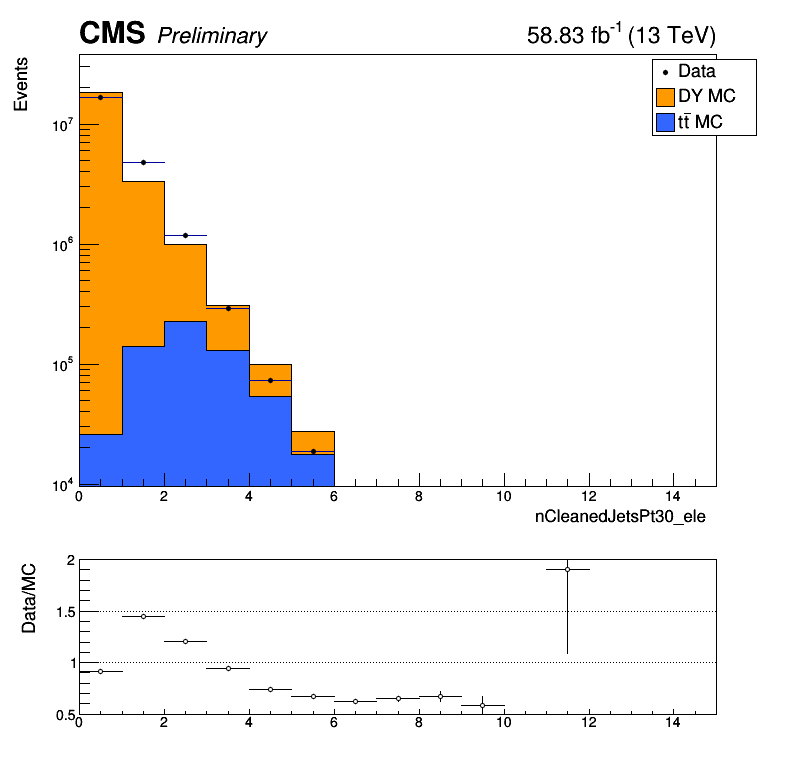
\includegraphics[width=0.49\linewidth]{Figures/Jets/nCleanedJetsPt30_ele.png} 
%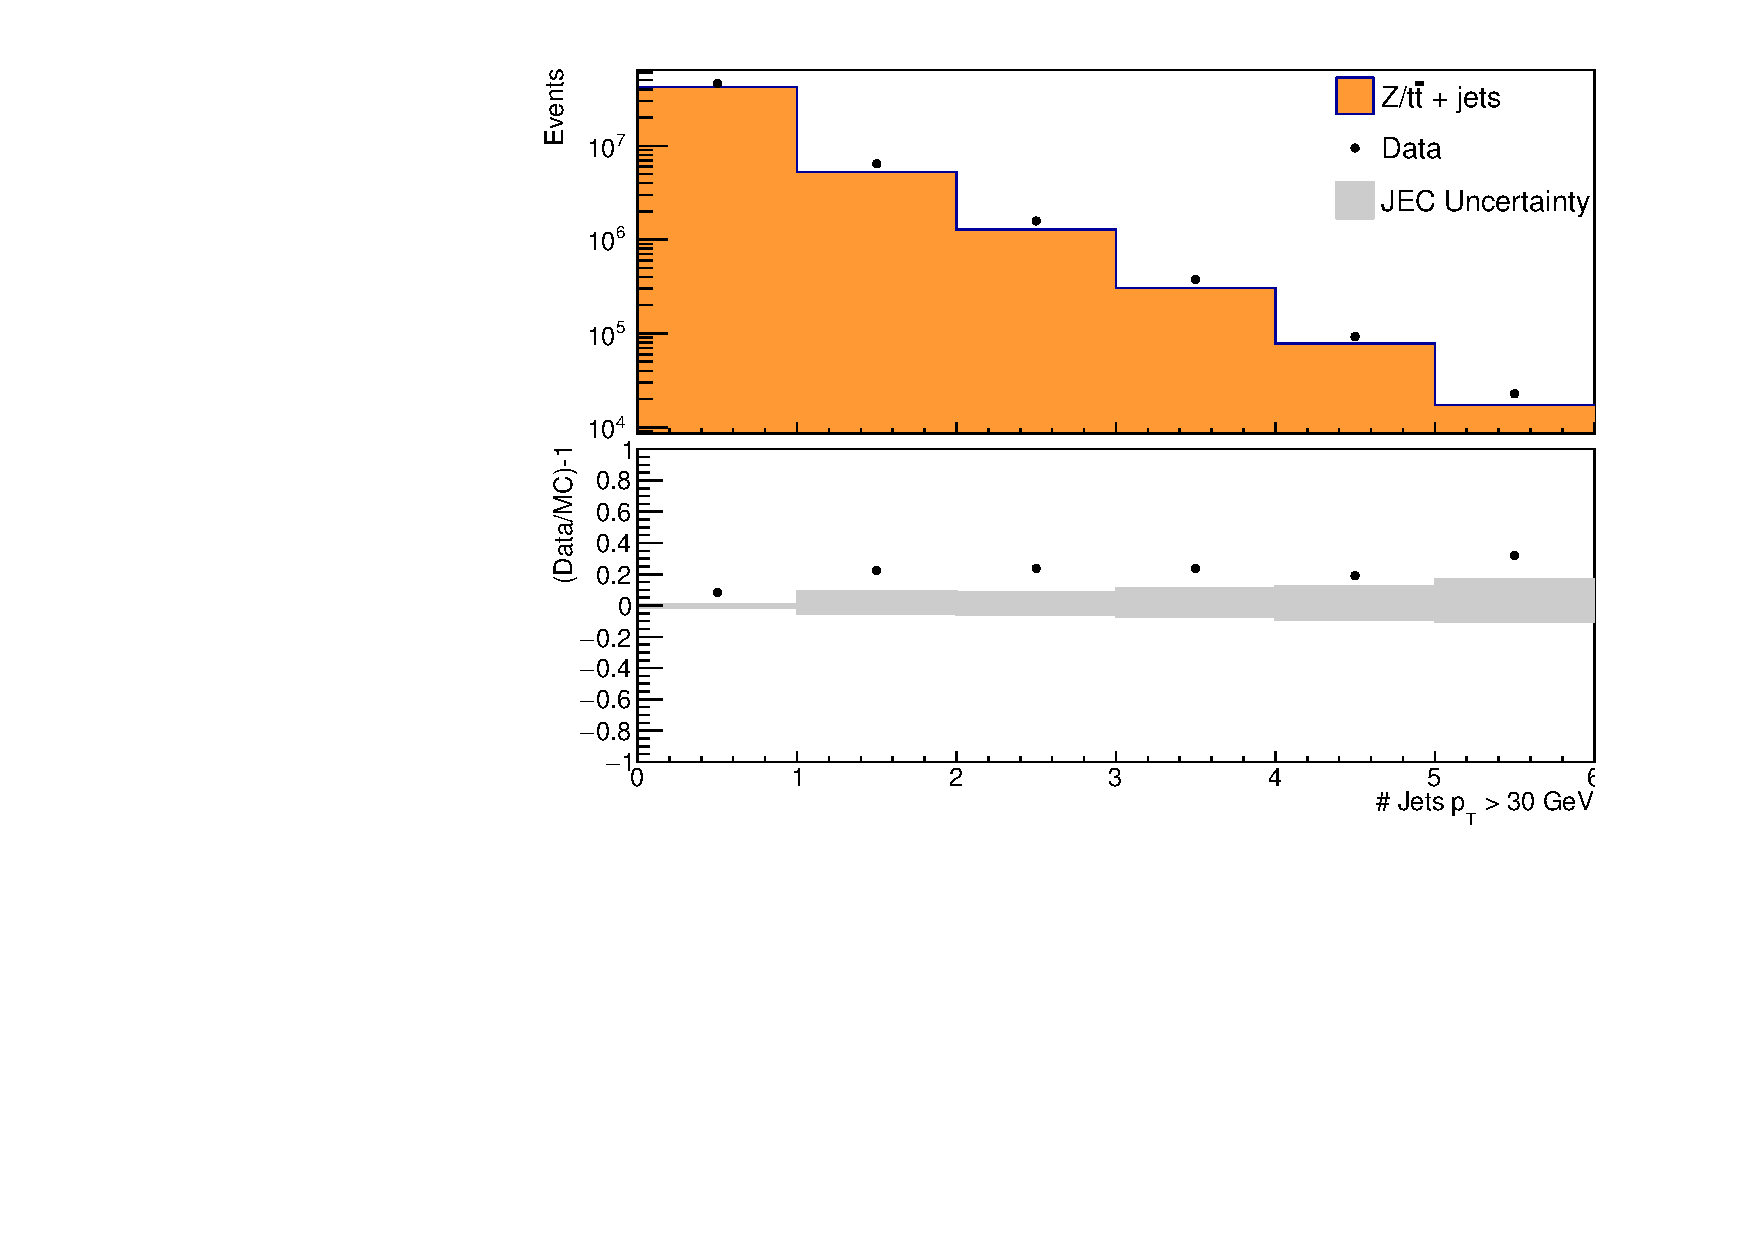
\includegraphics[width=0.69\linewidth]{Figures/Jets/nCleanedJetsPt30.pdf} \\
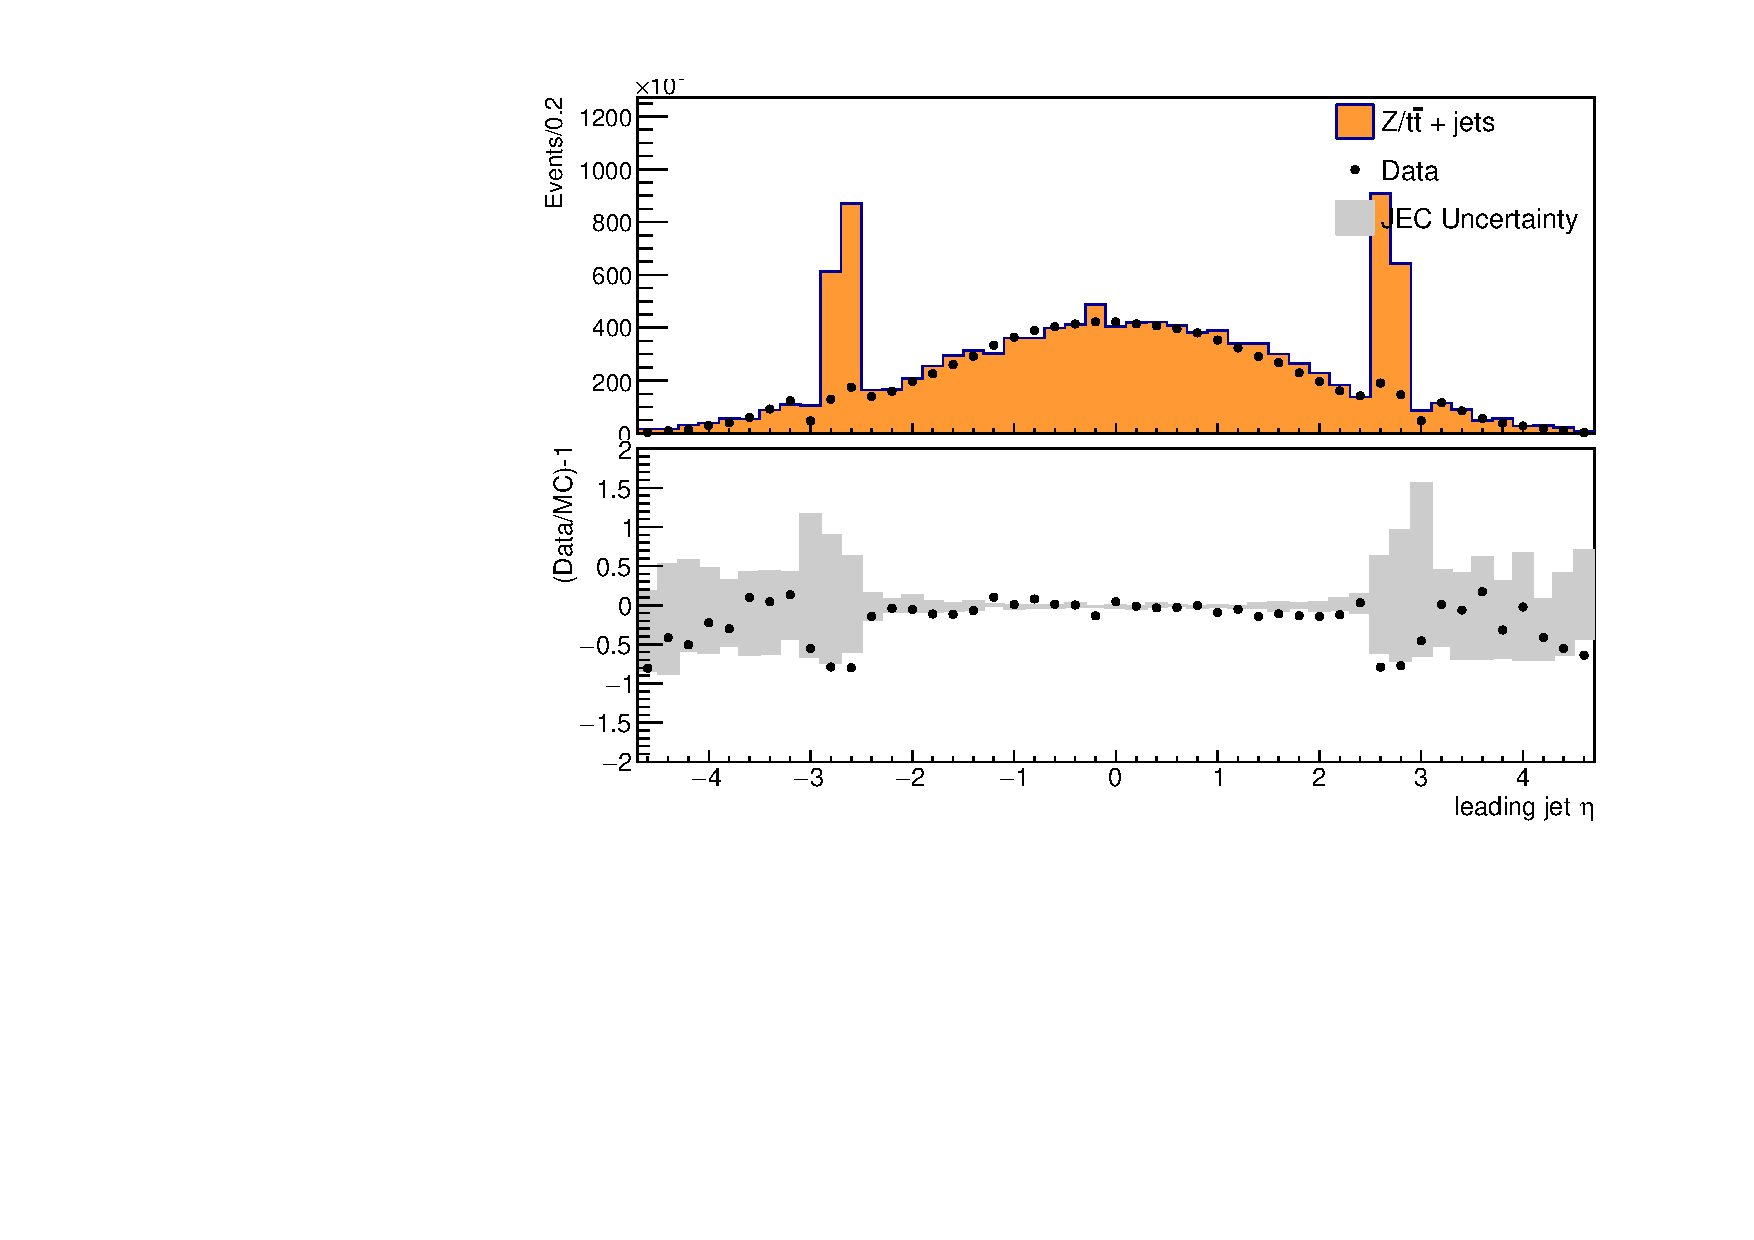
\includegraphics[width=0.69\linewidth]{Figures/Jets/leadingJet_Eta.pdf} 
%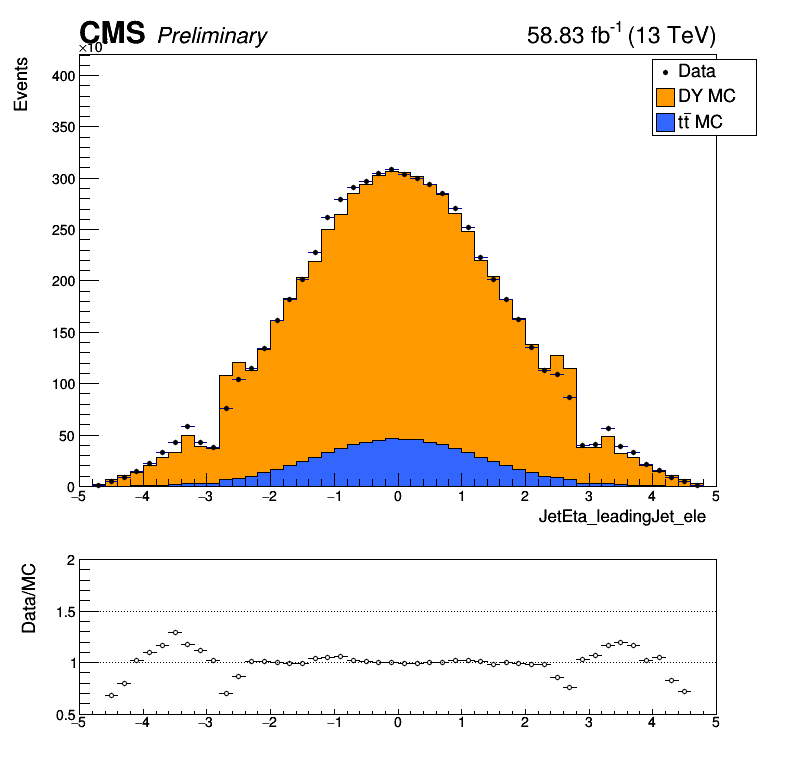
\includegraphics[width=0.49\linewidth]{Figures/Jets/JetEta_leadingJet_ele.png} \\ 
%\includegraphics[width=0.49\linewidth]{Figures/Jets/Histo_etaj1_2mu_dataeff.pdf}
\caption{Comparison of data with MC for leading jet $\eta$ in Z$\rightarrow \ell\ell$ +jets.
%for number of jets with $p_T>30$~GeV (top) and 
% (left) and Z$\rightarrow\mu\mu$ + jets events (right). 
MC is normalized to data. Jet ID and Jet PUID are applied. MC samples include DY and ttbar. Data/MC ratio plots are shown in the bottom of each plots, together with the uncertainties (shaded histograms) from Jet Energy Corrections.
%\textbf{FIXME: Add the uncertainty band in the ratio plot.}
\label{fig:jets}}
\end{figure}

%\begin{figure}[!h]
%\centering
%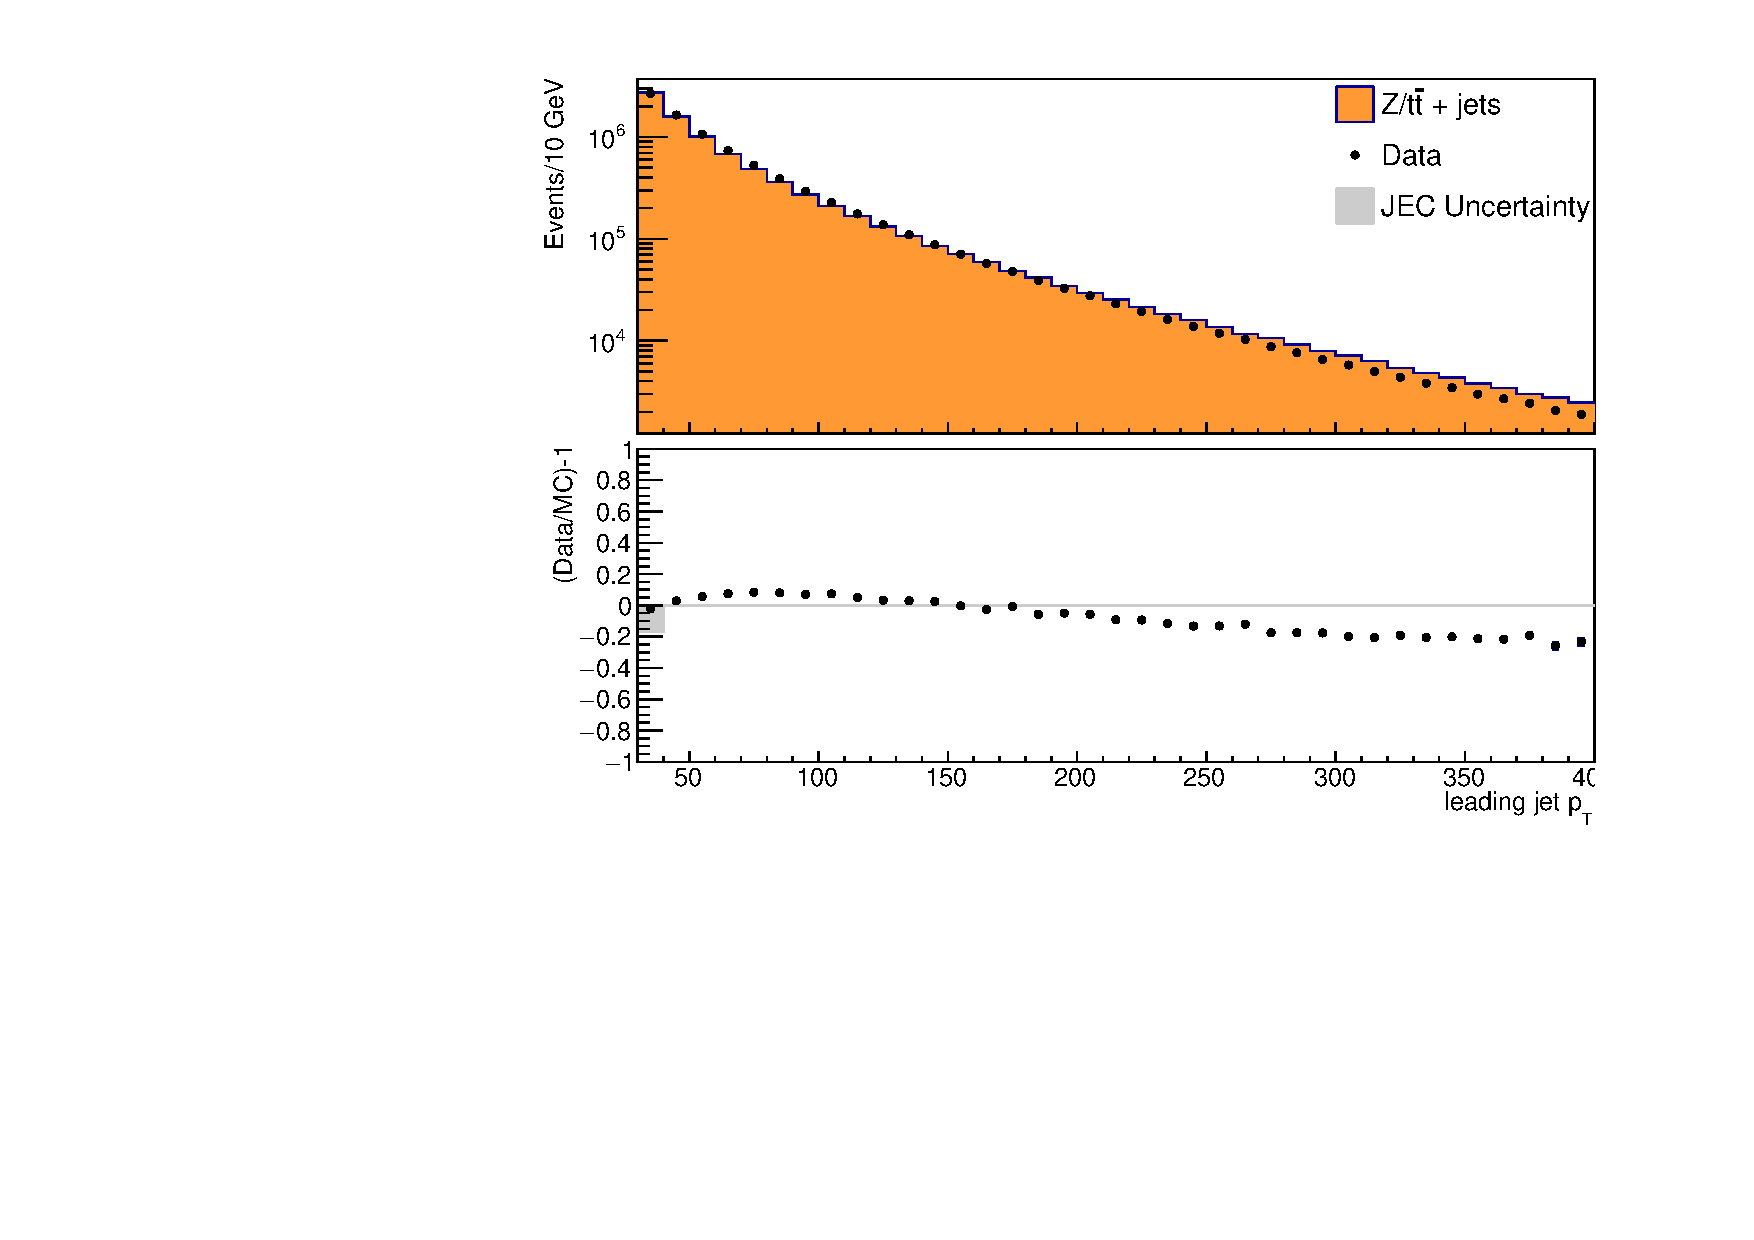
\includegraphics[width=0.69\linewidth]{Figures/Jets/leadingJet_Pt.pdf} \\
%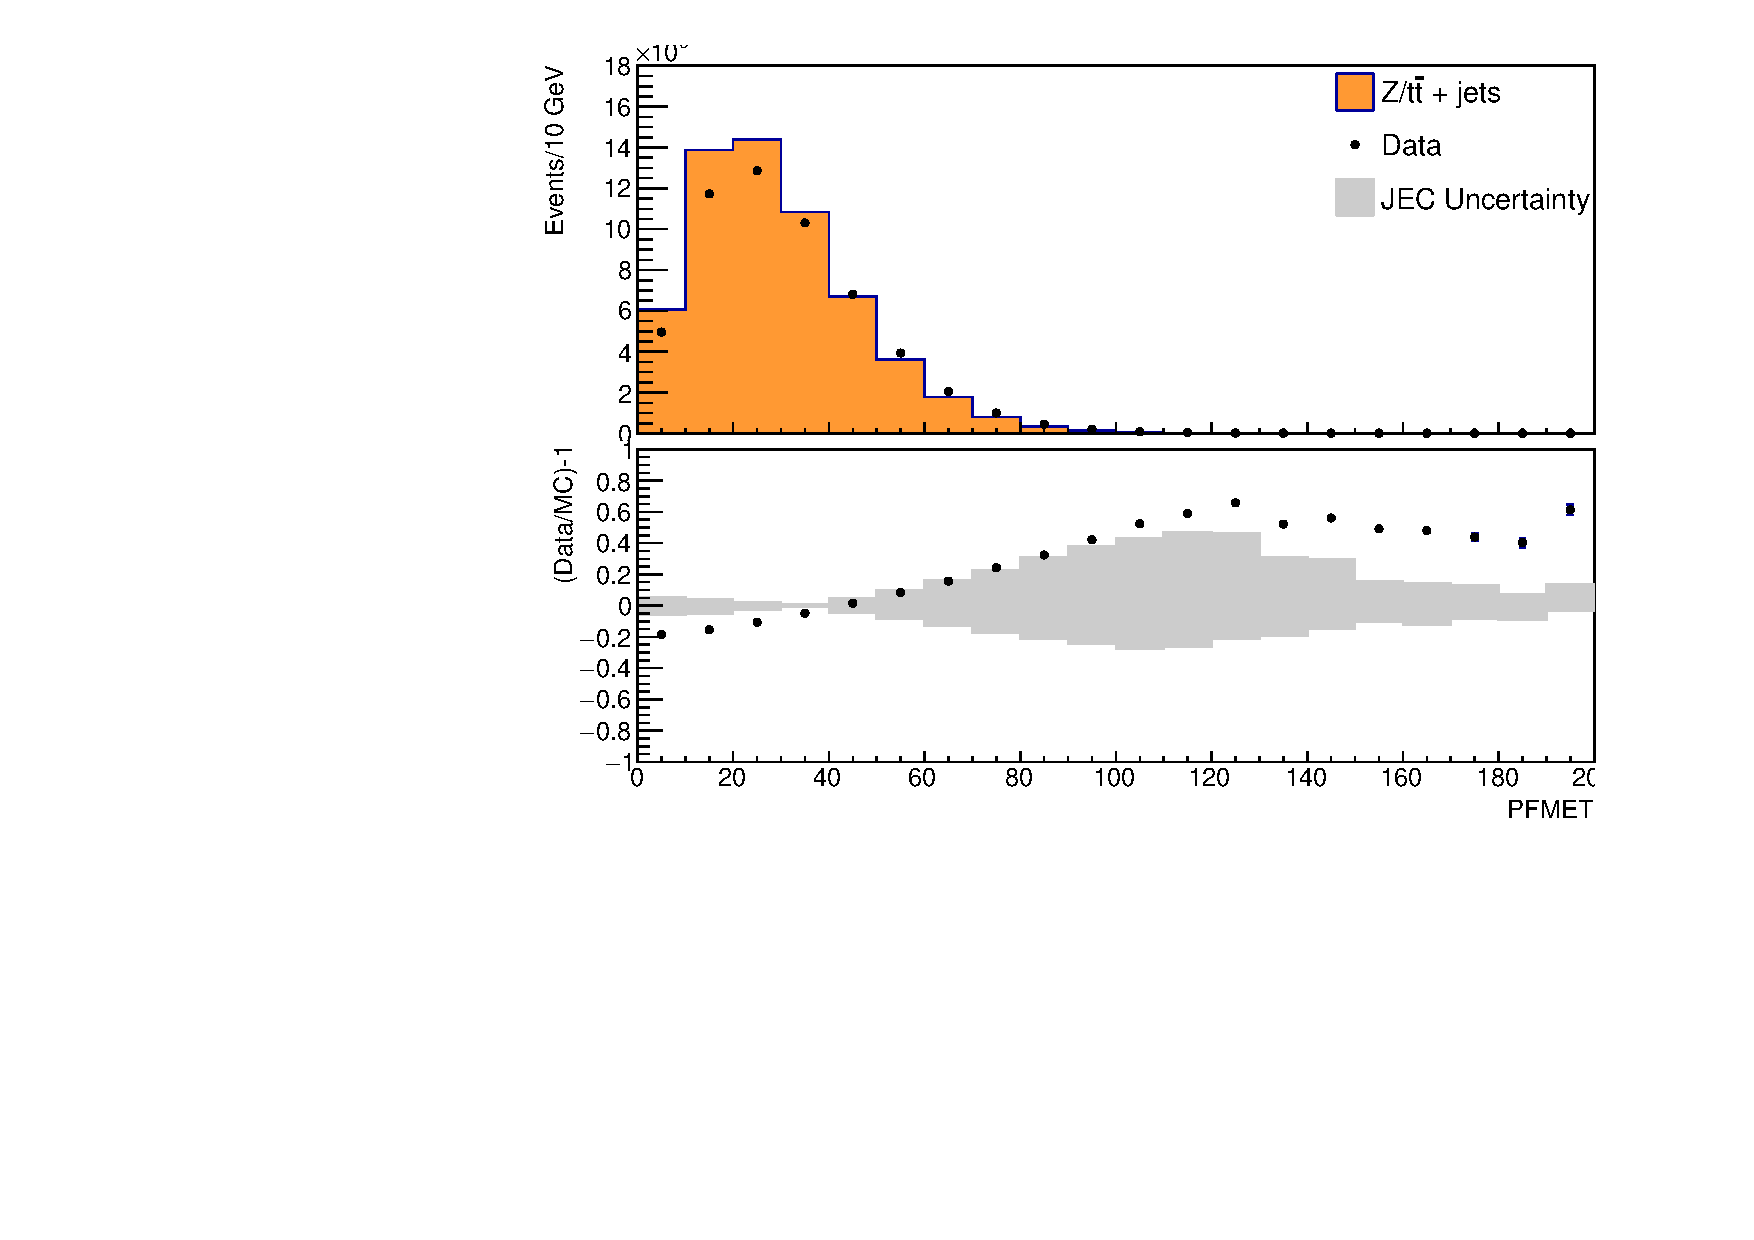
\includegraphics[width=0.69\linewidth]{Figures/Jets/PFMET.pdf} 
%\caption{Comparison between data and MC for the leading jet $p_T$ (left) and the PFMET with 
%Jet ID and Jet PUID applied. MC samples include DY and ttbar. MC is normalized to data. Data/MC ratio plots are shown in the bottom of each plots, together with the uncertainties (shaded histograms) from Jet Energy Corrections.
%\textbf{FIXME: Add the uncertainty band in the ratio plot.}
%\label{fig:met}}
%\end{figure}

%Horns around $\eta$~3 can be seen. It actually happens that Jet PUID and Jet ID were not applied in the plots above. 
%We thus reprocessed part of the data (Run C only) and the Drell-Yan MC with the latest recommendations for the JetMET POG and we obtained the plots on the Fig~\ref{fig:jetsID}:
 
%\begin{figure}[!h]
%\centering
%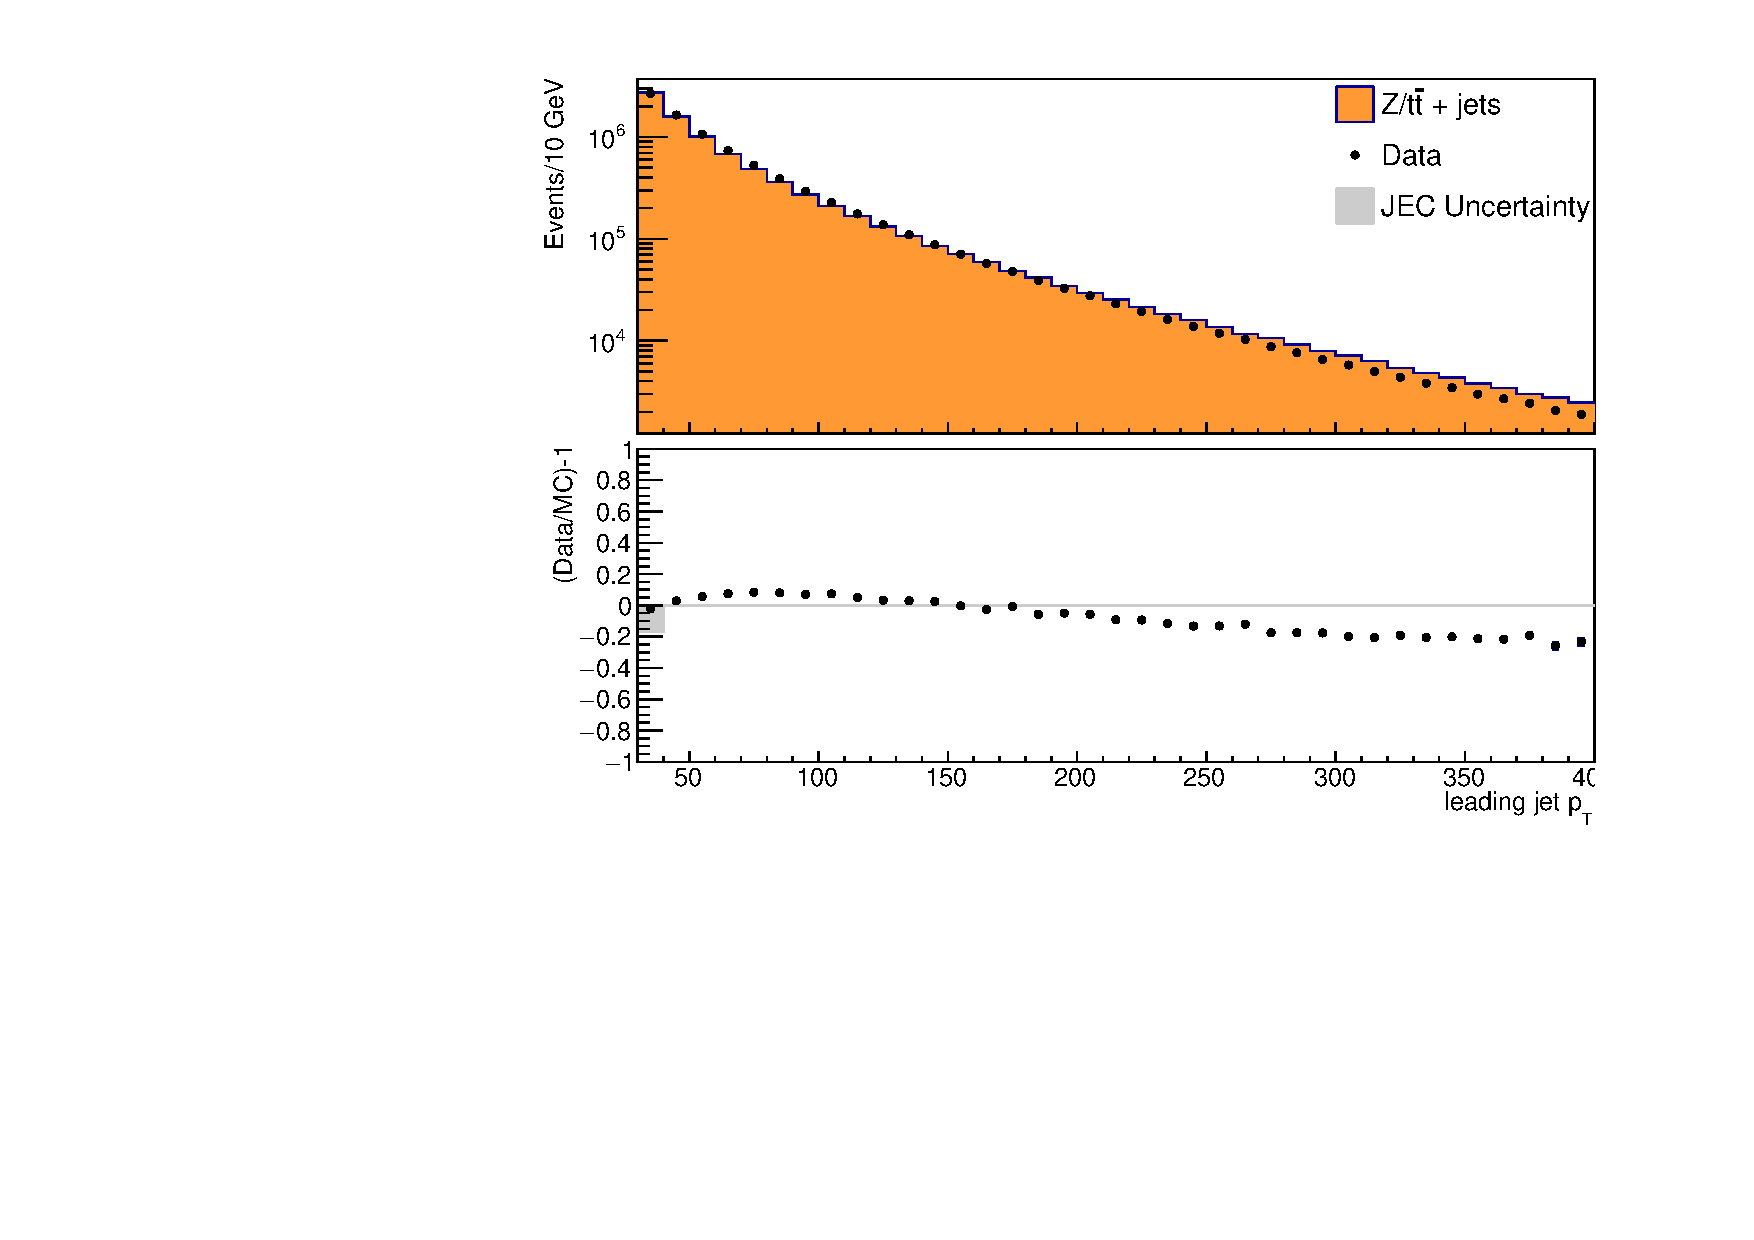
\includegraphics[width=0.4\linewidth]{Figures/Jets/leadingJet_Pt.pdf} %isto_etaj1_2e_dataeff.pdf}
%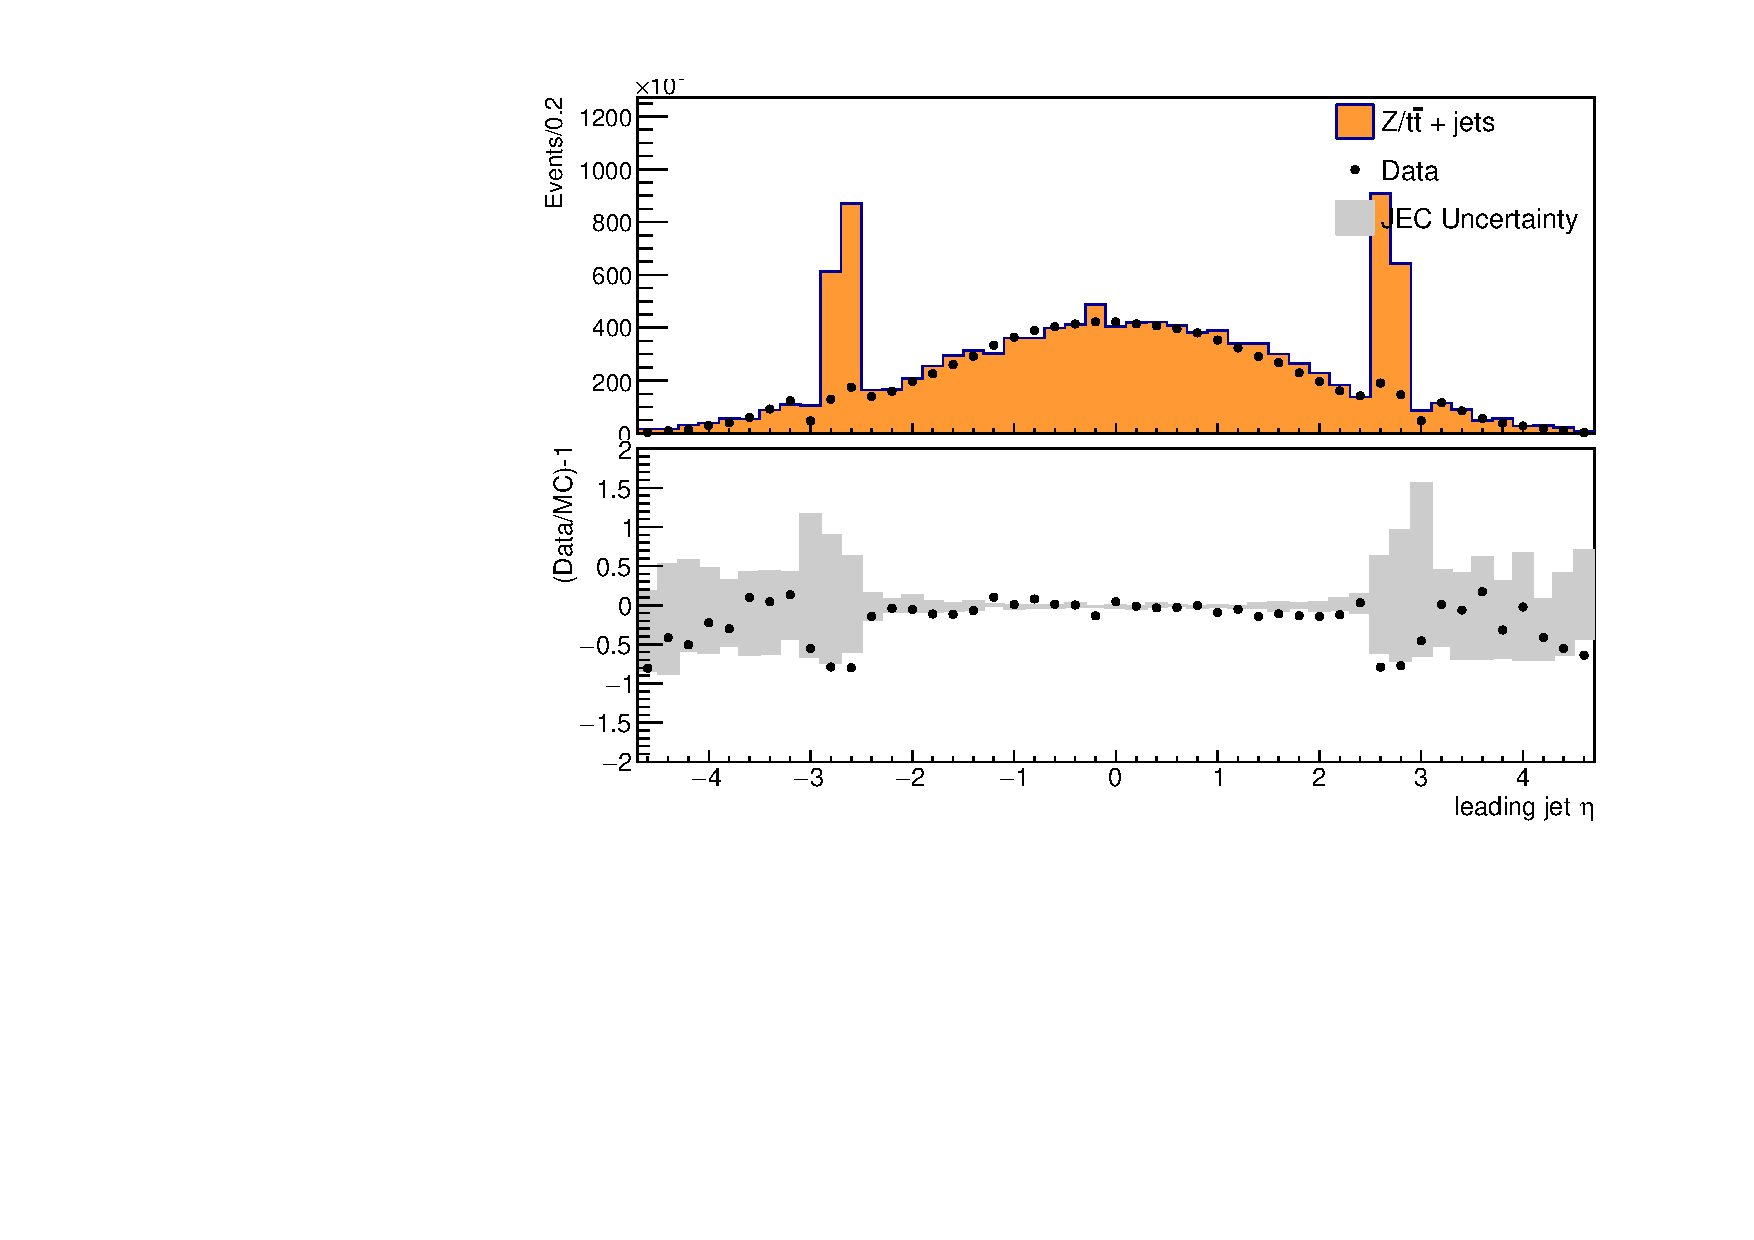
\includegraphics[width=0.4\linewidth]{Figures/Jets/leadingJet_Eta.pdf} \\
%\includegraphics[width=0.4\linewidth]{Figures/Jets/leadingJet_Phi.pdf}
%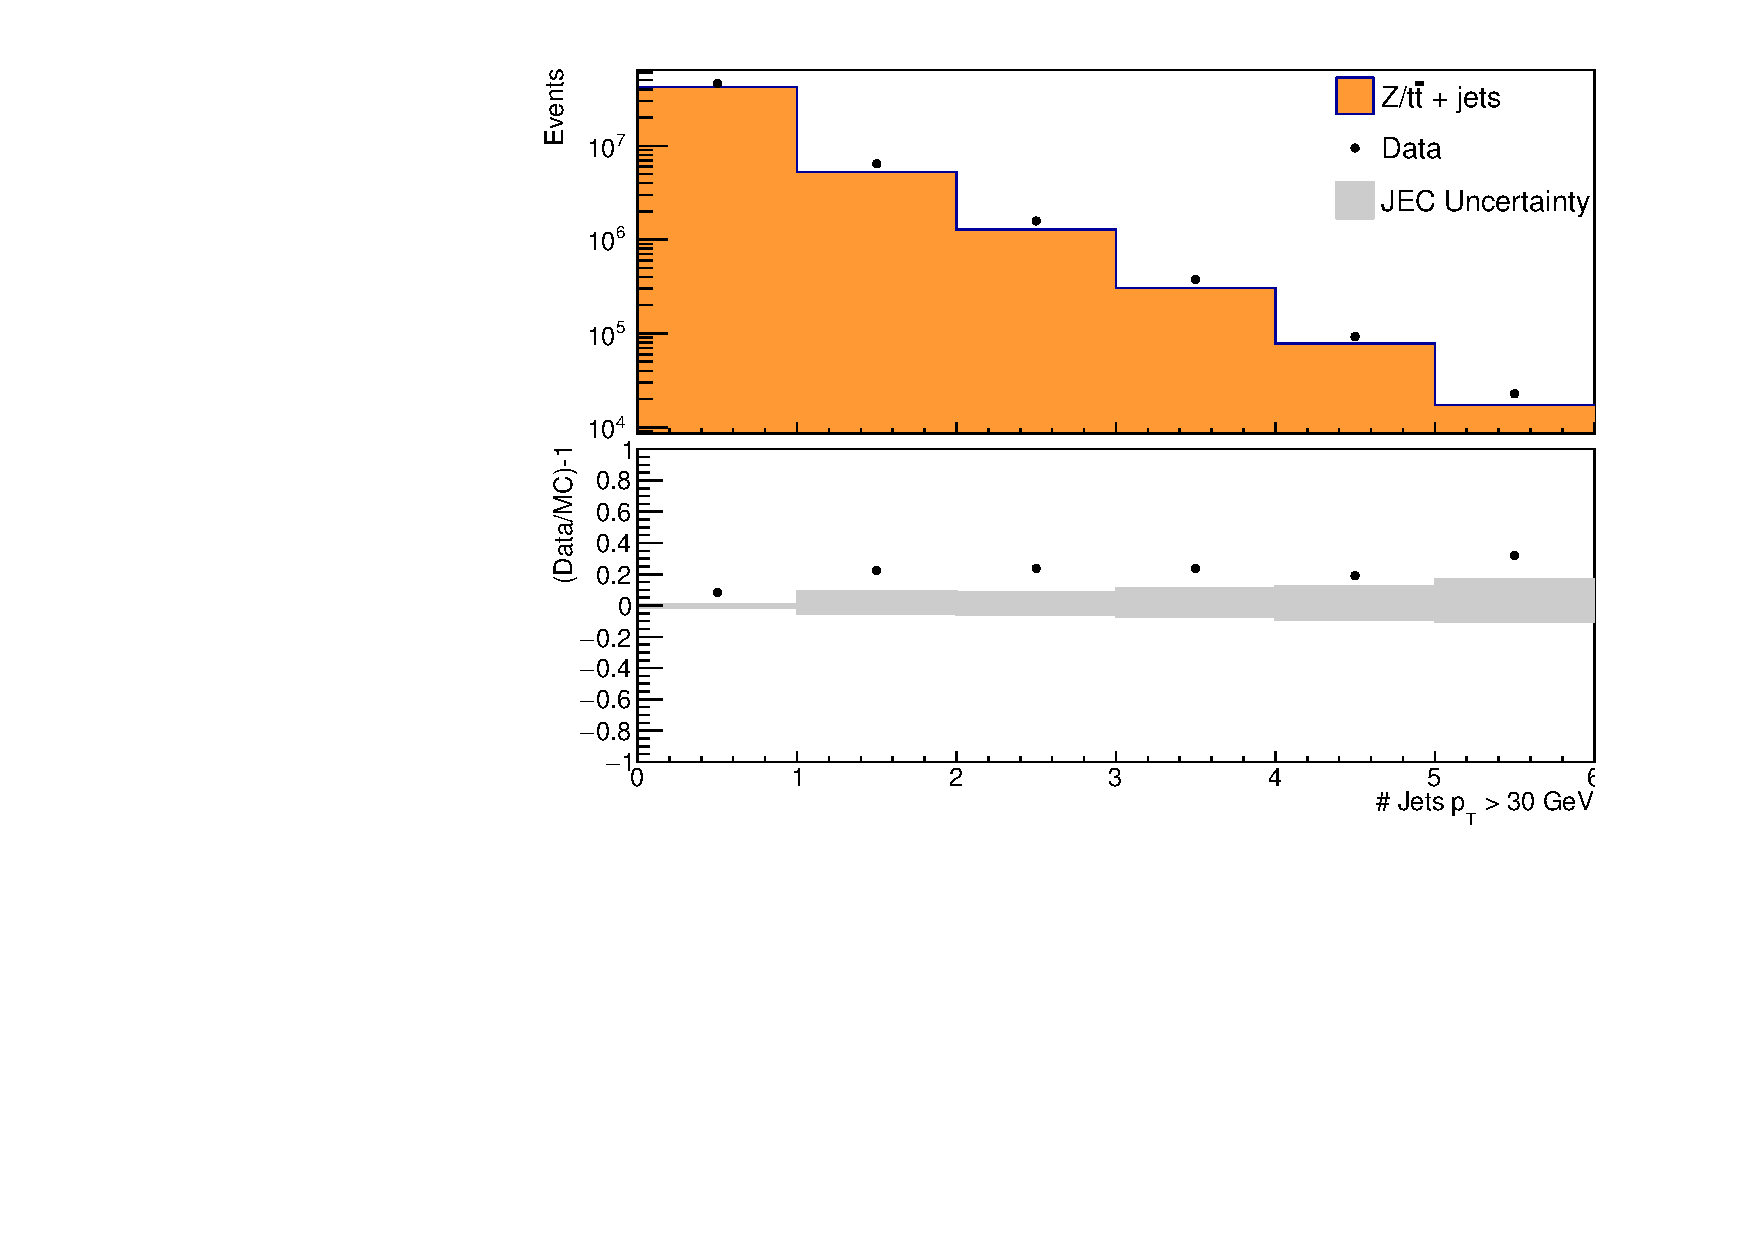
\includegraphics[width=0.4\linewidth]{Figures/Jets/nCleanedJetsPt30.pdf} \\
%\includegraphics[width=0.4\linewidth]{Figures/Jets/leadingJet_Btag.pdf}
%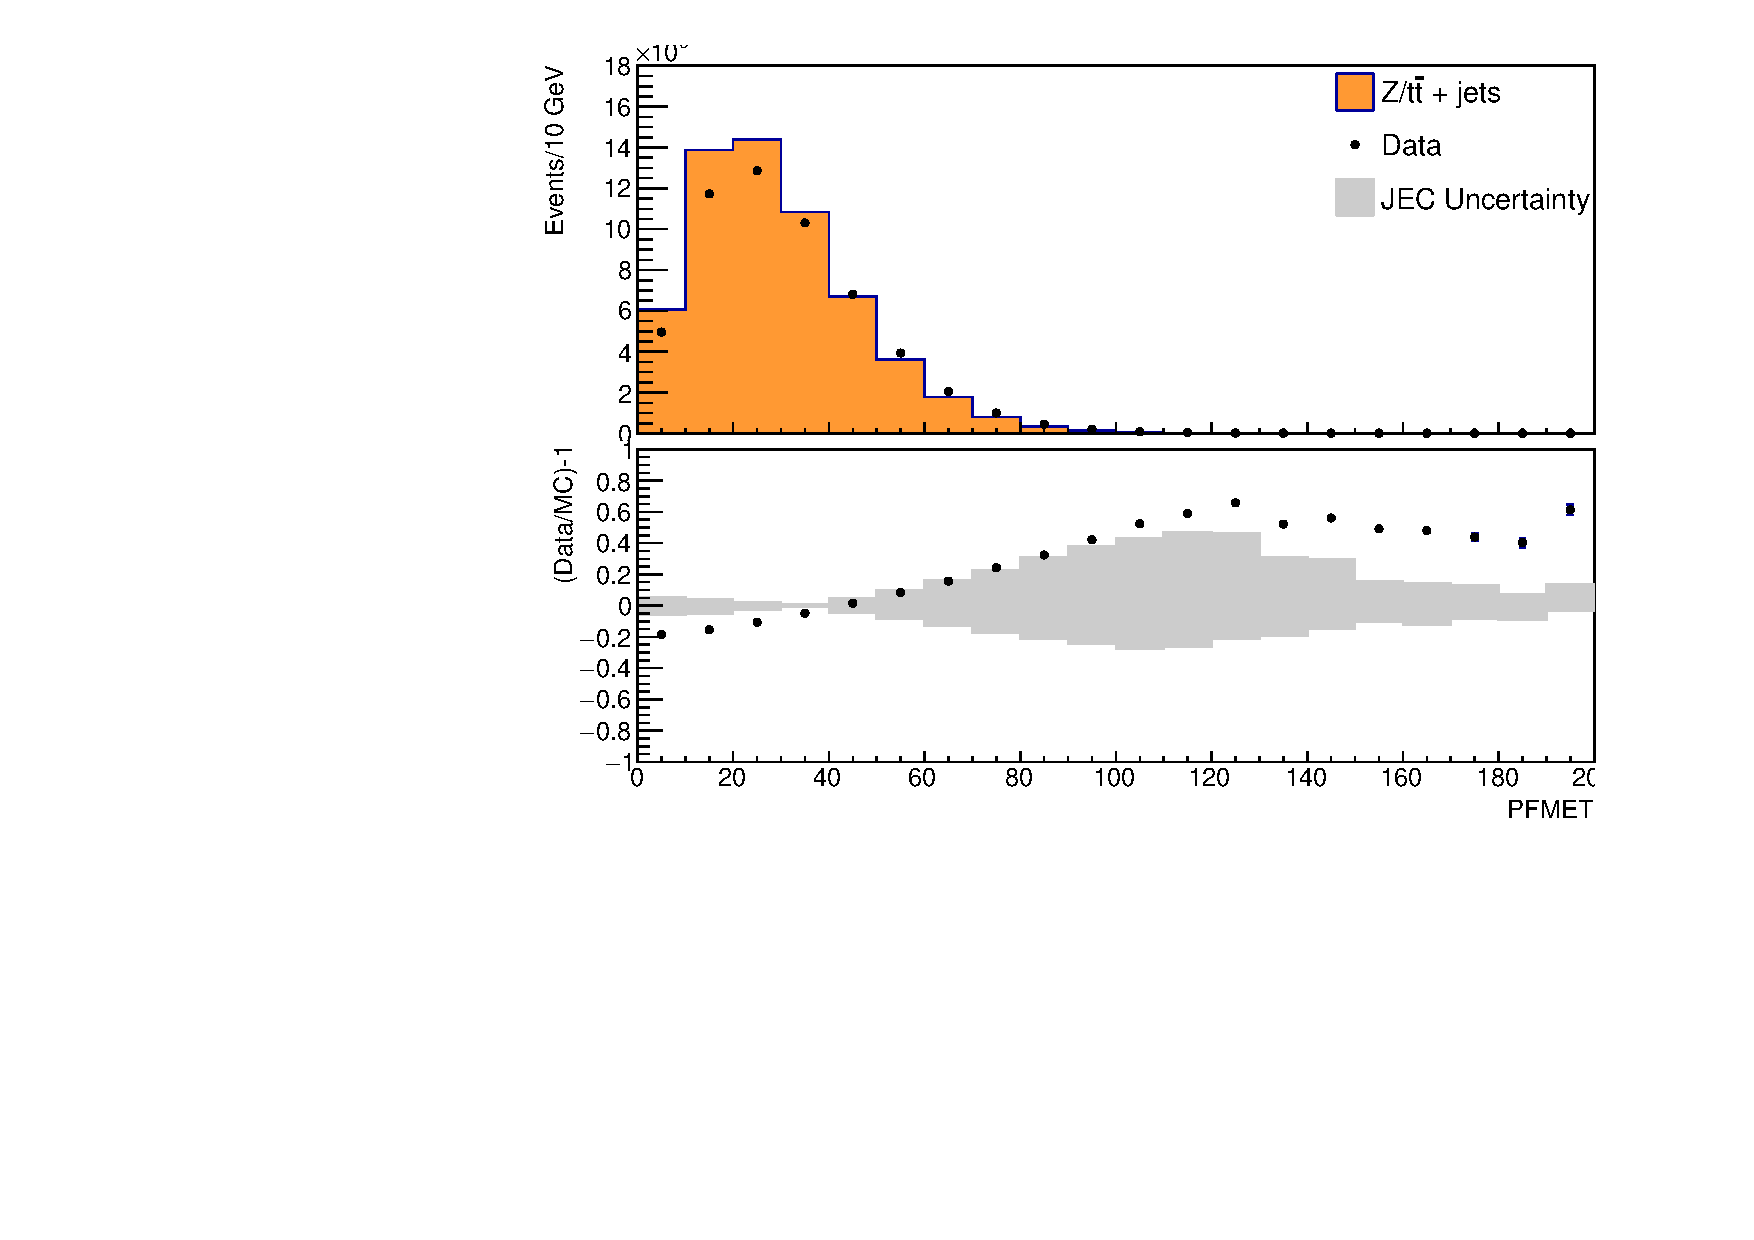
\includegraphics[width=0.4\linewidth]{Figures/Jets/PFMET.pdf}  \\
%\includegraphics[width=0.49\linewidth]{Figures/Jets/Histo_etaj1_2mu_dataeff.pdf}
%\caption{Comparison between data (RunC only) and MC for leading jet $p_T$ (top left), leading jet $\eta$ (top right), leading jet $\phi$ (middle left), number of jets with $p_T>30$~GeV (middle right), output of the b-tagger of the leading jet (bottom left) and PFMET (bottom right) in Z + jets events. Jet ID and Jet PUID are applied. $\ensuremath{\cPqt\bar{\cPqt}}$ MC sample is not included. 
%\label{fig:jetsID}}
%\end{figure}

%The agreement is now much better and only remain some mismatch in the tais, as one could expect for the missing contribution from $\ensuremath{\cPqt\bar{\cPqt}}$. While the results presented after do not include the JetPUID and JetID, we will include them in the next iteration, together with the final Scale Factors and object correction provided by the various POGs. 
